\begin{center}
\vspace*{0.1in}
\begin{Large}
\textbf{PRACTICA DE LABORATORIO N° 03:} \\
\textbf{(Creando un Reporte Interactivo en Power BI)} \\
\end{Large}
\end{center}
\begin{document}
\section{OBJETIVO:}
\item{
Desarrollar el Informe de Labratorio 02 de Creando un Reporte Interactivo en Power BI}
\section{REQUERIMIENTOS}
\begin{itemize}

Conocimientos
Para el desarrollo de esta práctica se requerirá de los siguientes conocimientos básicos:
\\- Conocimientos básicos de administración de base de datos Microsoft SQL Server.
\\- Conocimientos básicos de SQL.

Software
Asimismo se necesita los siguientes aplicativos:
\\- Microsoft SQL Server 2016 o superior
\\- Base de datos AdventureWorksLT2016 o superior
\\- Tener los archivos de recursos del laboratorio.
\\- Power BI Desktop.
\\- Tener una cuenta Microsoft registrada en el Portal de Power Bi

\end{itemize}

\section{CONSIDERACIONES INICIALES}
\item{Generar una carpeta o directorio Power BI en un lugar accesible para guardar los resultados de la práctica.}\\
\\\\\\\\\\\\\\\\\\\\\\\\\\\\
\section{DESARROLLO}

\subsection{Actividad No 01 – DESARROLLO1}

Ejercicio 1  Conectar a datos existentes \\
	\begin{center}
	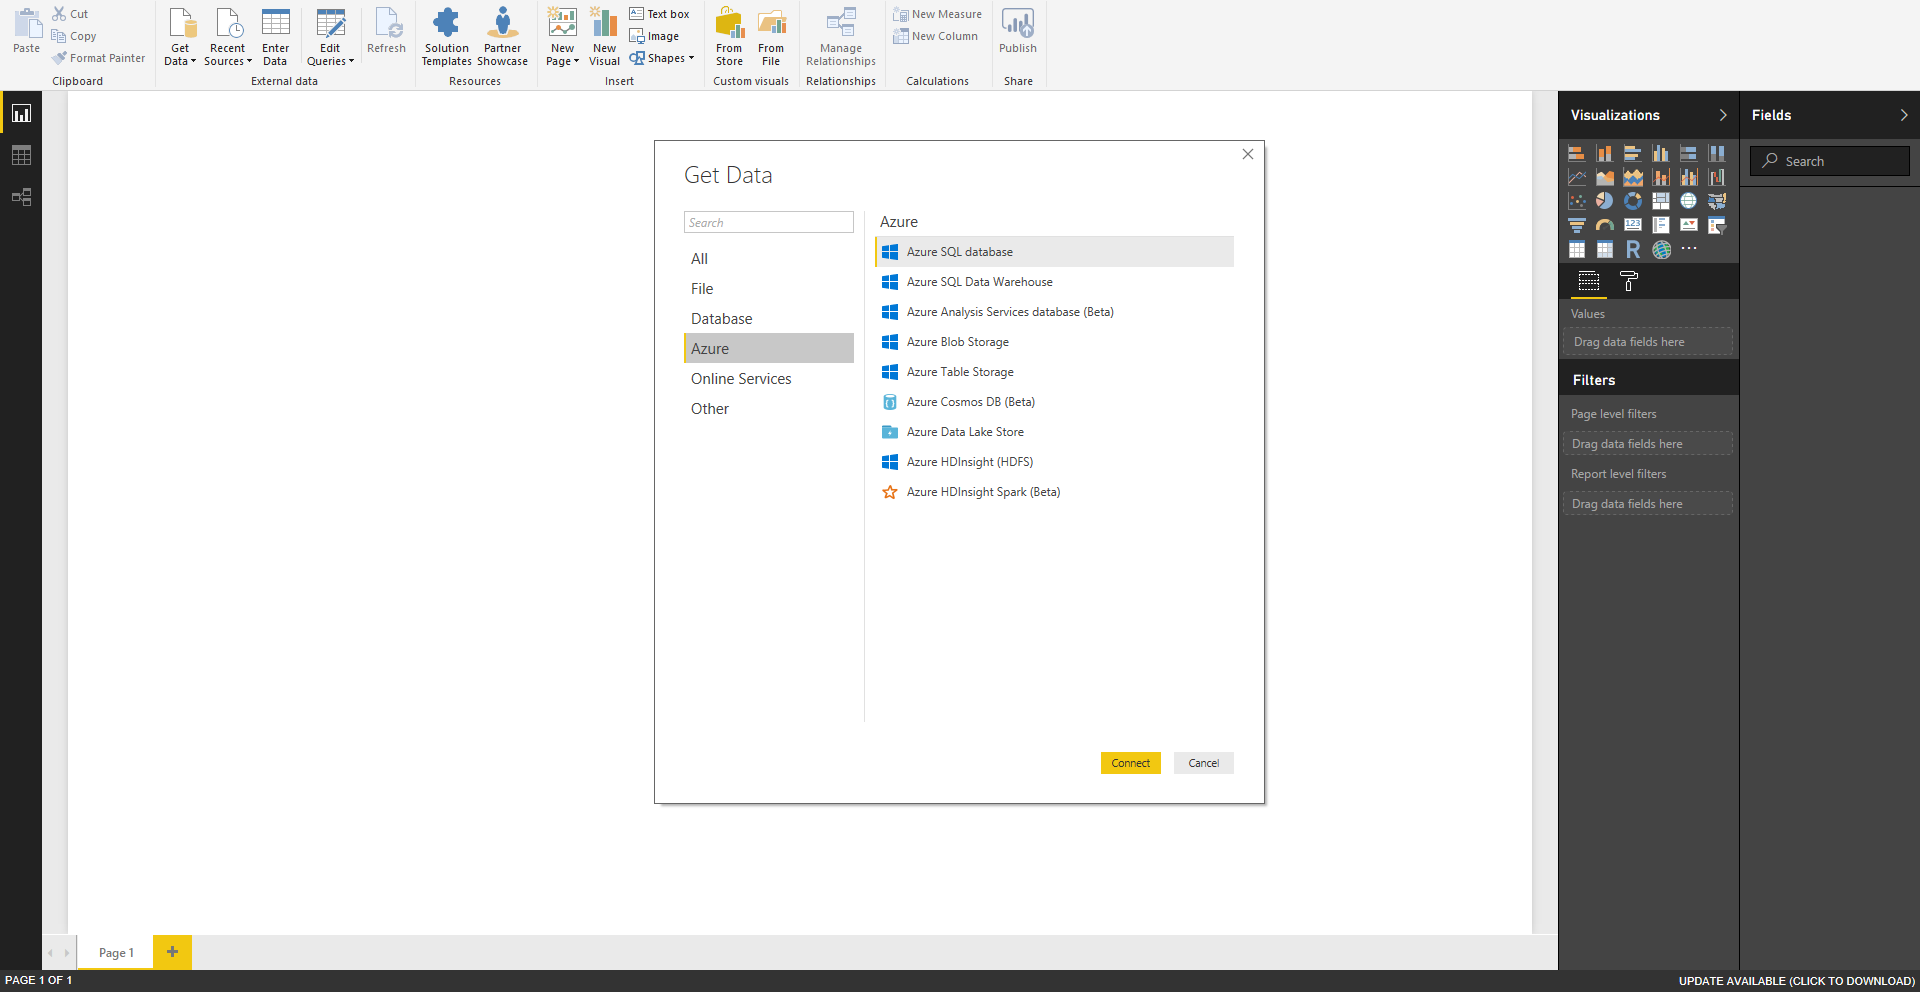
\includegraphics[width=15cm]{./Imagenes/EJER1T1(1)}
	\end{center}	

	\begin{center}
	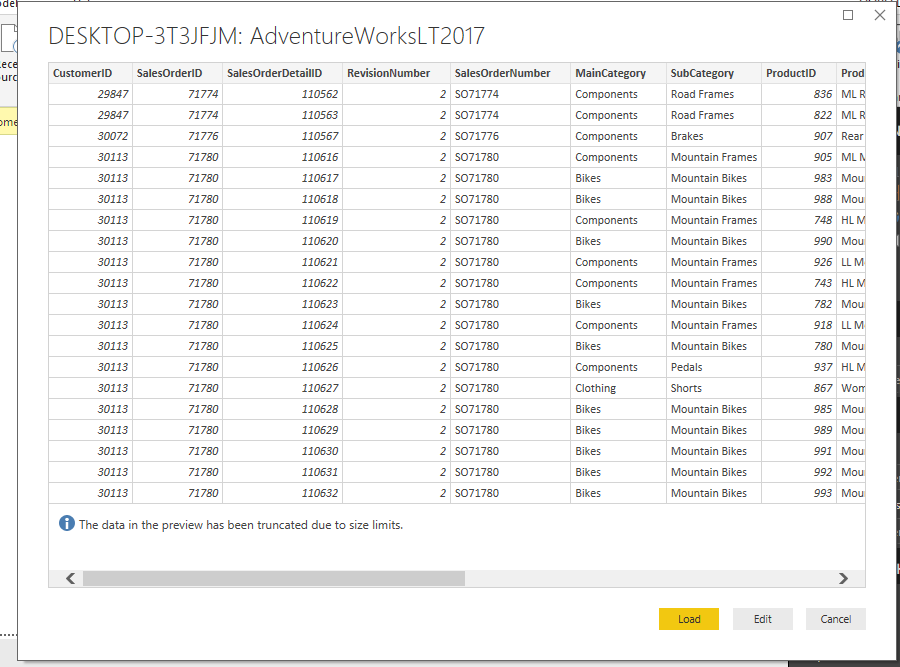
\includegraphics[width=15cm]{./Imagenes/EJER1T1(4)}
	\end{center}
	\newpage
Ejercicio 2: Shape Data\\
	\begin{center}
	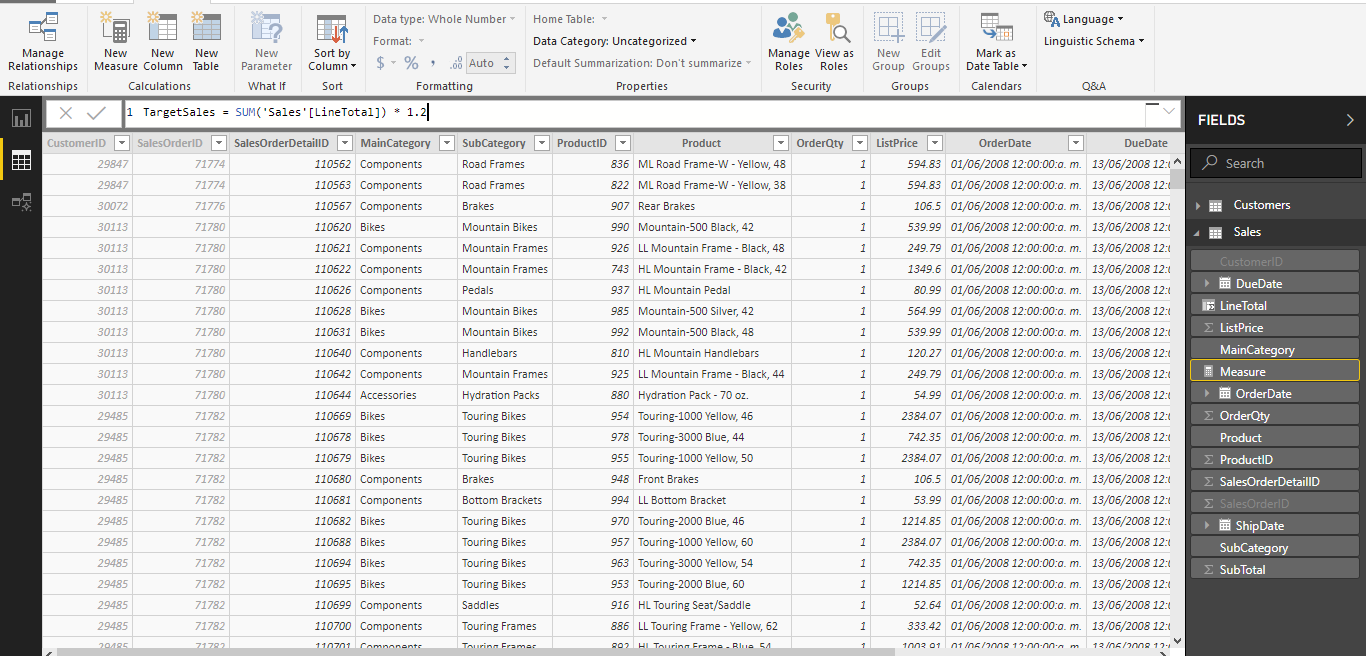
\includegraphics[width=15cm]{./Imagenes/EJER1T2(1)}
	\end{center}	

	

	\begin{center}
	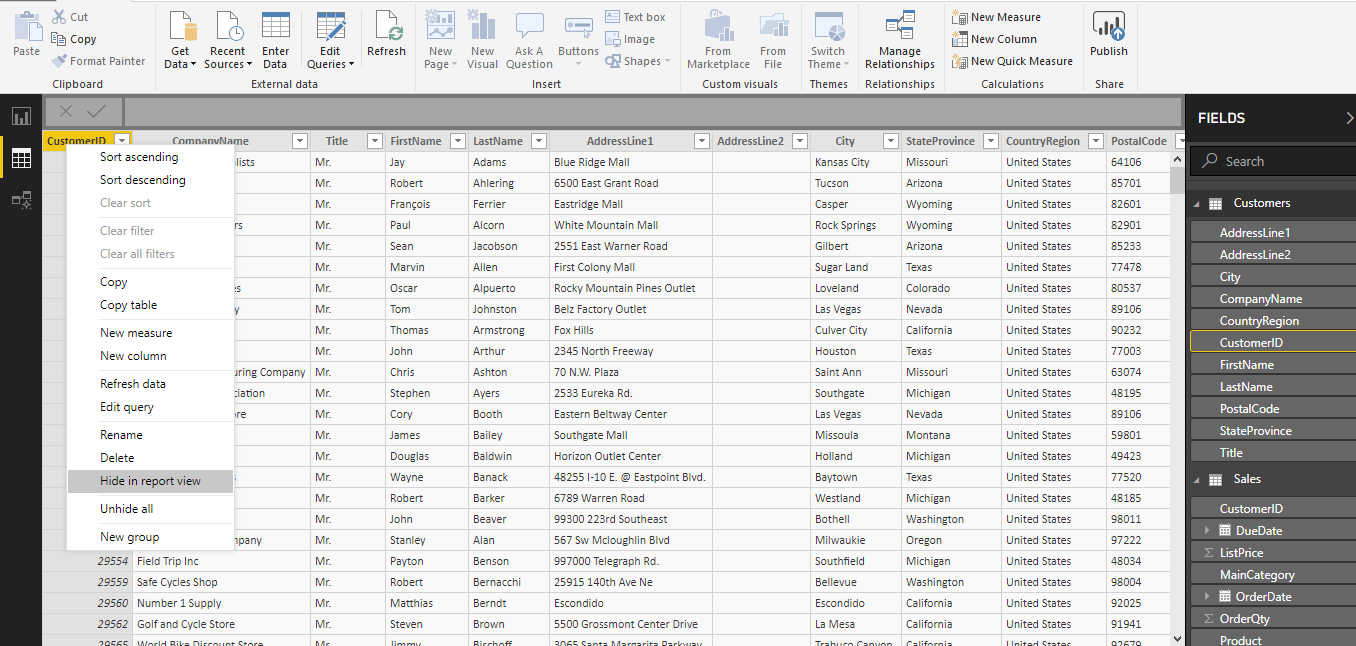
\includegraphics[width=15cm]{./Imagenes/EJER1T2(3)}
	\end{center}	
\newpage

	\begin{center}
	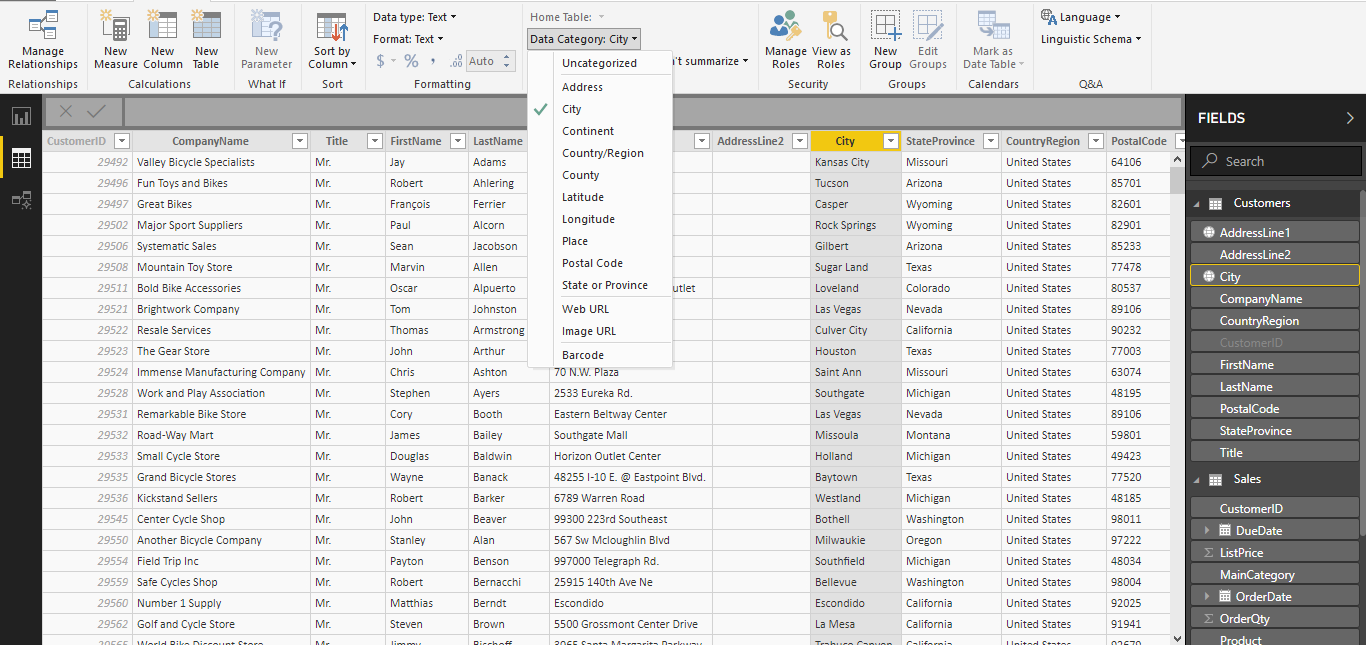
\includegraphics[width=15cm]{./Imagenes/EJER1T2(5)}
	\end{center}	


	

	\begin{center}
	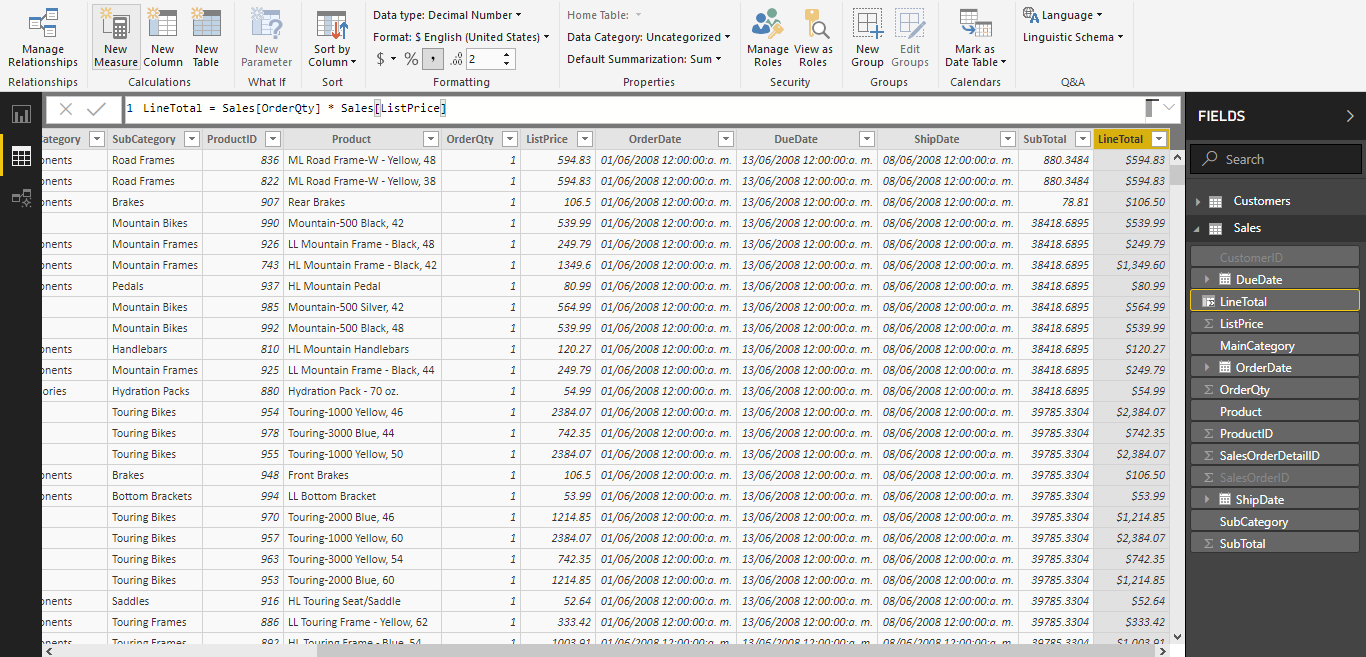
\includegraphics[width=15cm]{./Imagenes/EJER1T2(8)}
	\end{center}	
\newpage
Ejercicio 3: Combine Data\\
	\begin{center}
	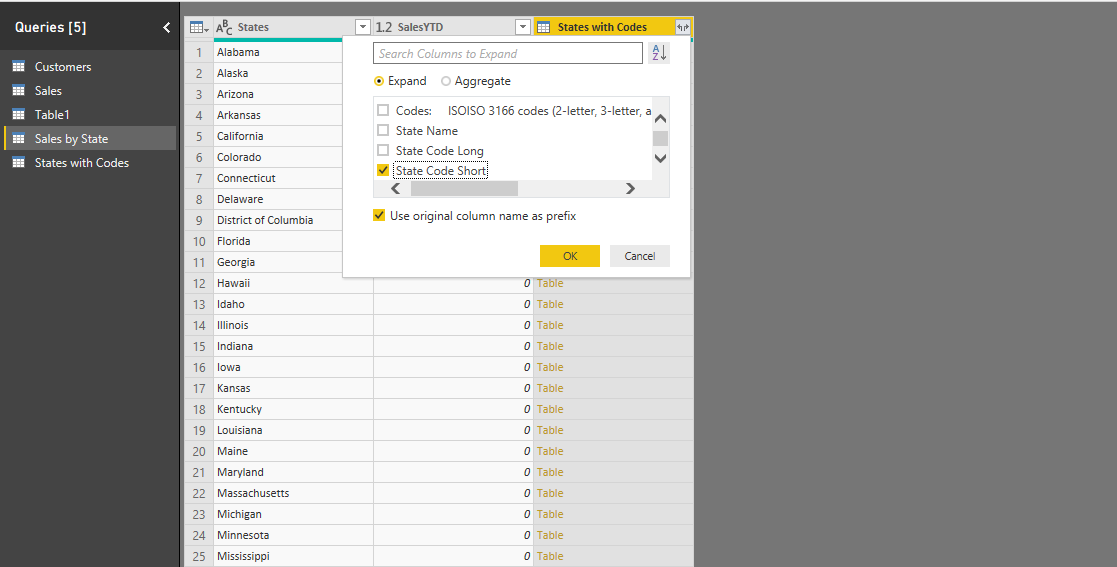
\includegraphics[width=15cm]{./Imagenes/EJER1T3(1)}
	\end{center}	

	\begin{center}
	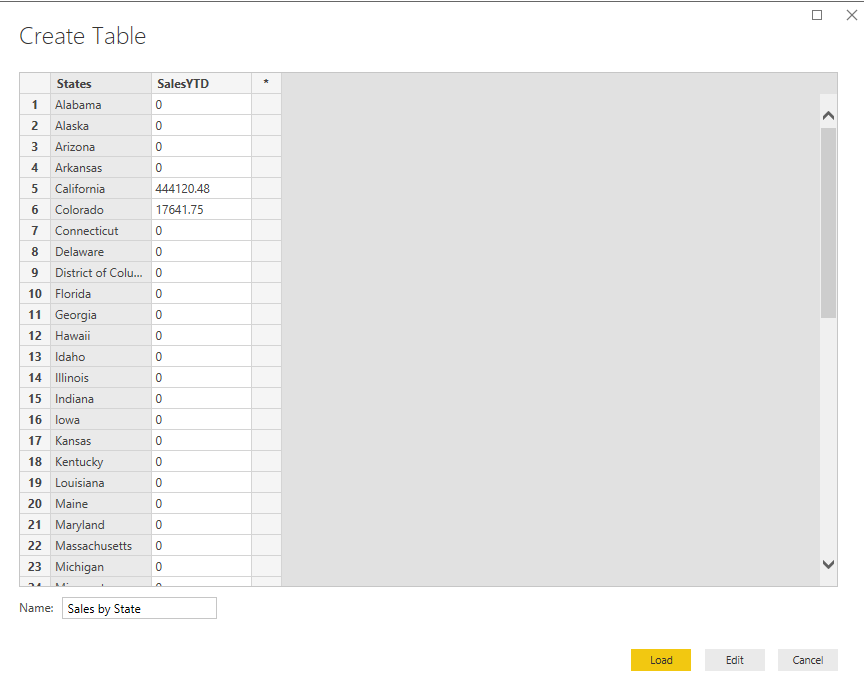
\includegraphics[width=15cm]{./Imagenes/EJER1T3(3)}
	\end{center}	
\newpage
	

	\begin{center}
	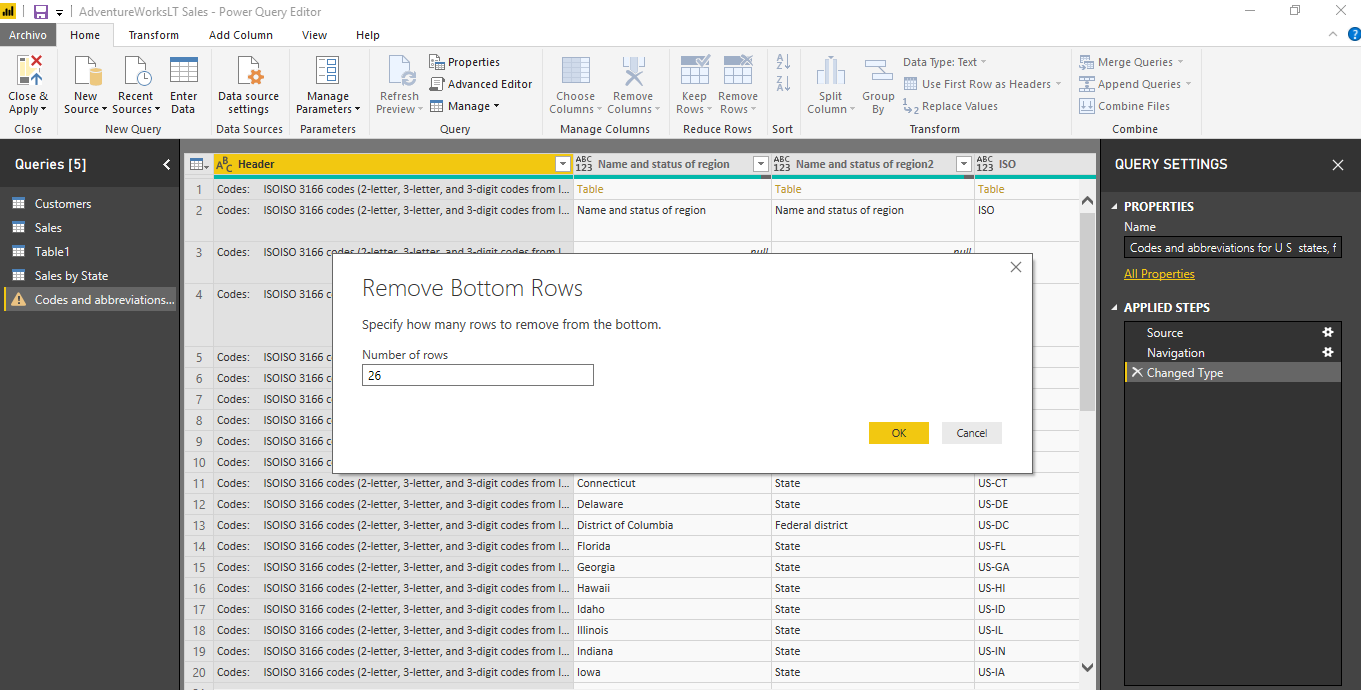
\includegraphics[width=15cm]{./Imagenes/EJER1T3(6)}
	\end{center}	
	

	\begin{center}
	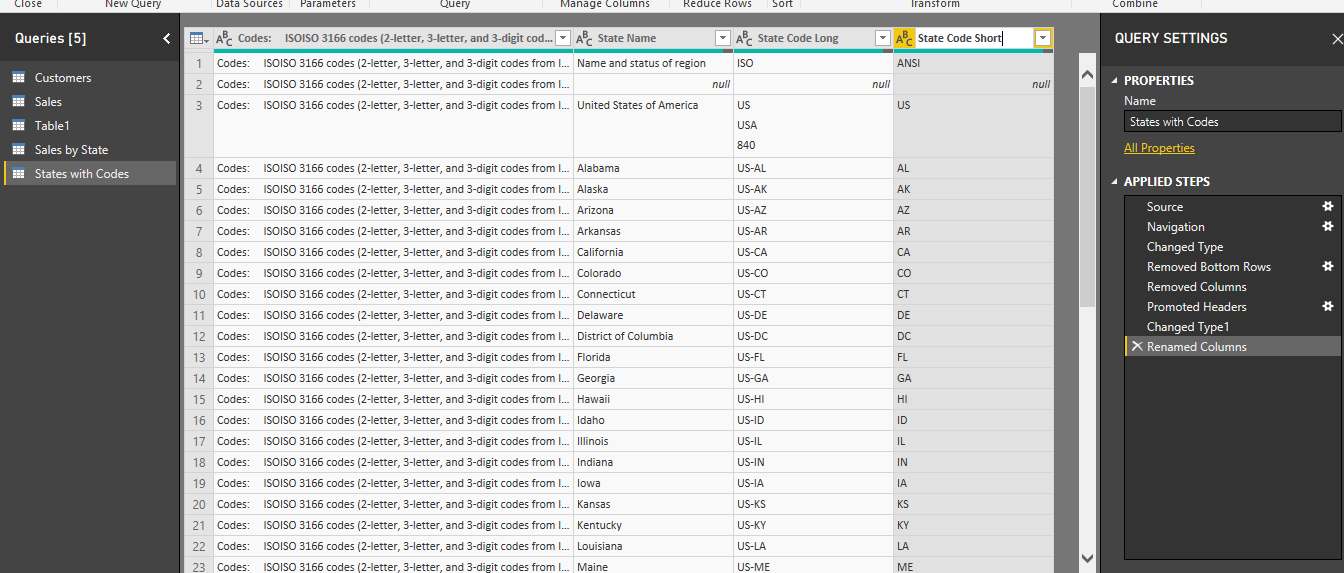
\includegraphics[width=15cm]{./Imagenes/EJER1T3(8)}
	\end{center}	
\newpage
	\begin{center}
	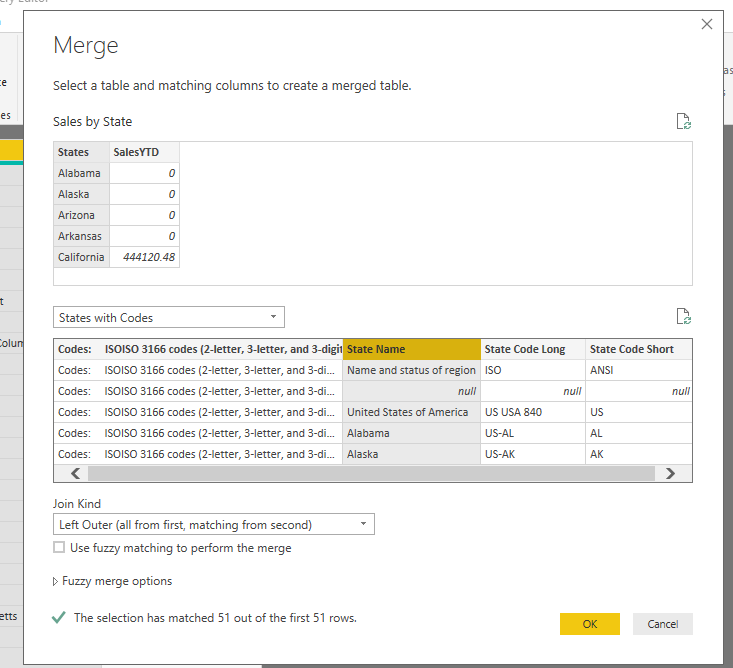
\includegraphics[width=15cm]{./Imagenes/EJER1T3(9)}
	\end{center}	


